\subsection{Privacy Provider}

\setcounter{figure}{8}  
\begin{figure}[!ht]
	\centering
	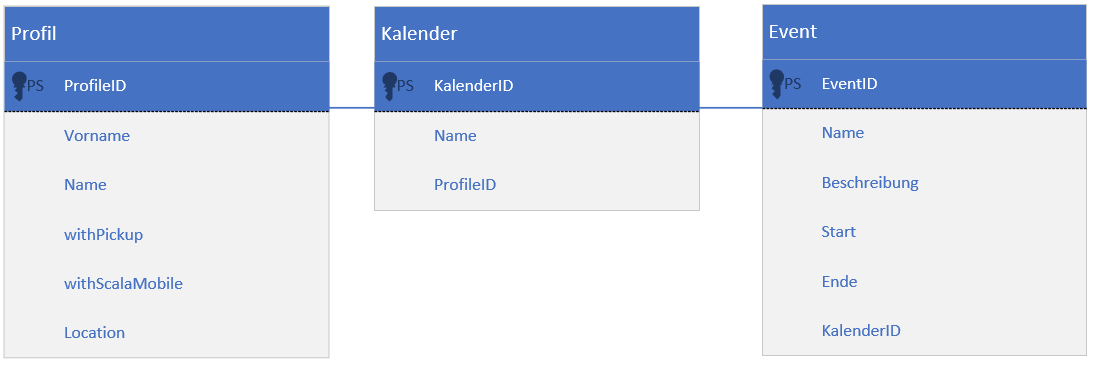
\includegraphics[width=1\linewidth]{Picture/Datenmodell}
	\caption[Datenmodell]{Datenmodell des Anwendungsfalls}
	\label{fig:datenmodell}
\end{figure}

In dem bereitgestellten Privacy Provider sollen Informationen zum Nutzerkontext gespeichert werden. Das Datenmodell ist speziell für die Anwendungsfälle beschrieben. Dabei werden personenbezogene Daten und freie Zeiten benötigt. Der Nutzerkontext wird durch dieses Datenmodell nur sehr eingeschränkt beschrieben. Allerdings kann das Datenmodell erweitert werden.

In diesem Datenmodell, welches in Abbildung \ref{fig:datenmodell} aufgezeigt ist, kann der Benutzer verschiedene Profile auswählen. So kann der richtige Name angegeben oder die Identität hinter einen anderen Namen verborgen werden. In dem Profil werden Angaben zur Mobilität hinterlegt, z.B. ob ein Fahr-Service und ein Scala Mobile benötigt wird. Mit den Profildaten sind die Kalender verknüpft. Die Daten werden direkt vom Smartphone ausgelesen, aber es können auch weitere Online-Kalender hinzugefügt werden. Schließlich beinhaltet ein Kalender mehrere Events. Für den Ort gibt es das Location-Feld. Die Location kann über den GPS-Sensor bestimmt oder es kann ein Ort eingegeben werden.
